\documentclass{standalone}
\usepackage[T1]{fontenc}
\usepackage[latin2]{inputenc}
\usepackage[english]{babel}
\usepackage{tikz}
\usepackage{times}
\usetikzlibrary{calc,through,backgrounds,positioning,fit}
\usetikzlibrary{shapes,arrows,shadows}
 
\begin{document}

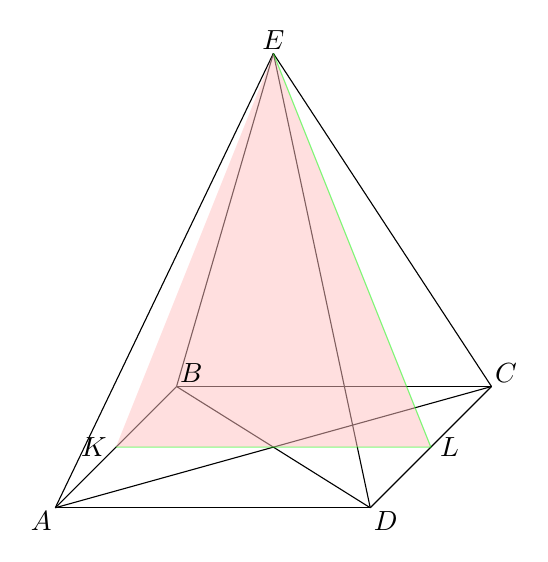
\begin{tikzpicture}[scale=1,inner sep=0.4mm]

\coordinate (A) at (0,0,4);
\coordinate (B) at (0,0,0);
\coordinate (C) at (4,0,0);
\coordinate (D) at (4,0,4);
\coordinate (E) at (2,5,2);
\coordinate (K) at (0,0,2);
\coordinate (L) at (4,0,2);

\draw[-] (A) to (E);
\draw[-] (A) to (B);
\draw[-] (A) to (C);
\draw[-] (A) to (D);
\draw[-] (C) to (B);
\draw[-] (C) to (D);
\draw[-] (C) to (E);
\draw[-] (B) to (E);
\draw[-] (B) to (D);
\draw[-] (D) to (E);

\fill[draw=green, fill=pink, opacity=0.5] (E) to (L) to (K);

\node at (A) [below left] {$A$};
\node at (D) [below right] {$D$};
\node at (B) [above right] {$B$};
\node at (C) [above right] {$C$};
\node at (E) [above] {$E$};
\node at (L) [right=2pt] {$L$};
\node at (K) [left=2pt] {$K$};

\end{tikzpicture}

\end{document}